\documentclass[10pt,a4paper]{article}
\usepackage[utf8]{inputenc}
\usepackage{amsmath}
\usepackage{amsfonts}
\usepackage{amssymb}
\usepackage{listings}
\usepackage{graphicx}
\graphicspath{ {../img/} }
\author{Gradey Cullins}
\title{Assignment 5}
\begin{document}
\maketitle

\section*{Explanation of Code}
The starting point of the submitted code is the script \emph{main.m}. \\

\noindent
To analytically solve and plot the solution to problem 1, run the function \emph{coffee\_cup\_solver.m}. This function utilizes the \emph{Tsexact} function, which provides the step-by-step numeric calculation of the cooling problem for each iteration. \\

\noindent
Problem 2 similarly utilizes the \emph{Tsexact} function in its calculation of the cooling problem and is solved using the \emph{forward\_eulers} script. \\

\noindent
Problem 3 through 6 use the \emph{ode23\_2} function.

\section{}
To solve problem one I implemented the \emph{Tsexact} function. The solution that I used is defined below: \\
\begin{lstlisting}
function Texact = Tsexact(Tenv, T0, R, t)    
    Texact = Tenv + (T0 - Tenv) .* exp(-R.*t);    
end
\end{lstlisting}

\clearpage

\noindent
The plot produced by running the provided code and named \emph{coffee\_cup\_solver.m} is also shown below:

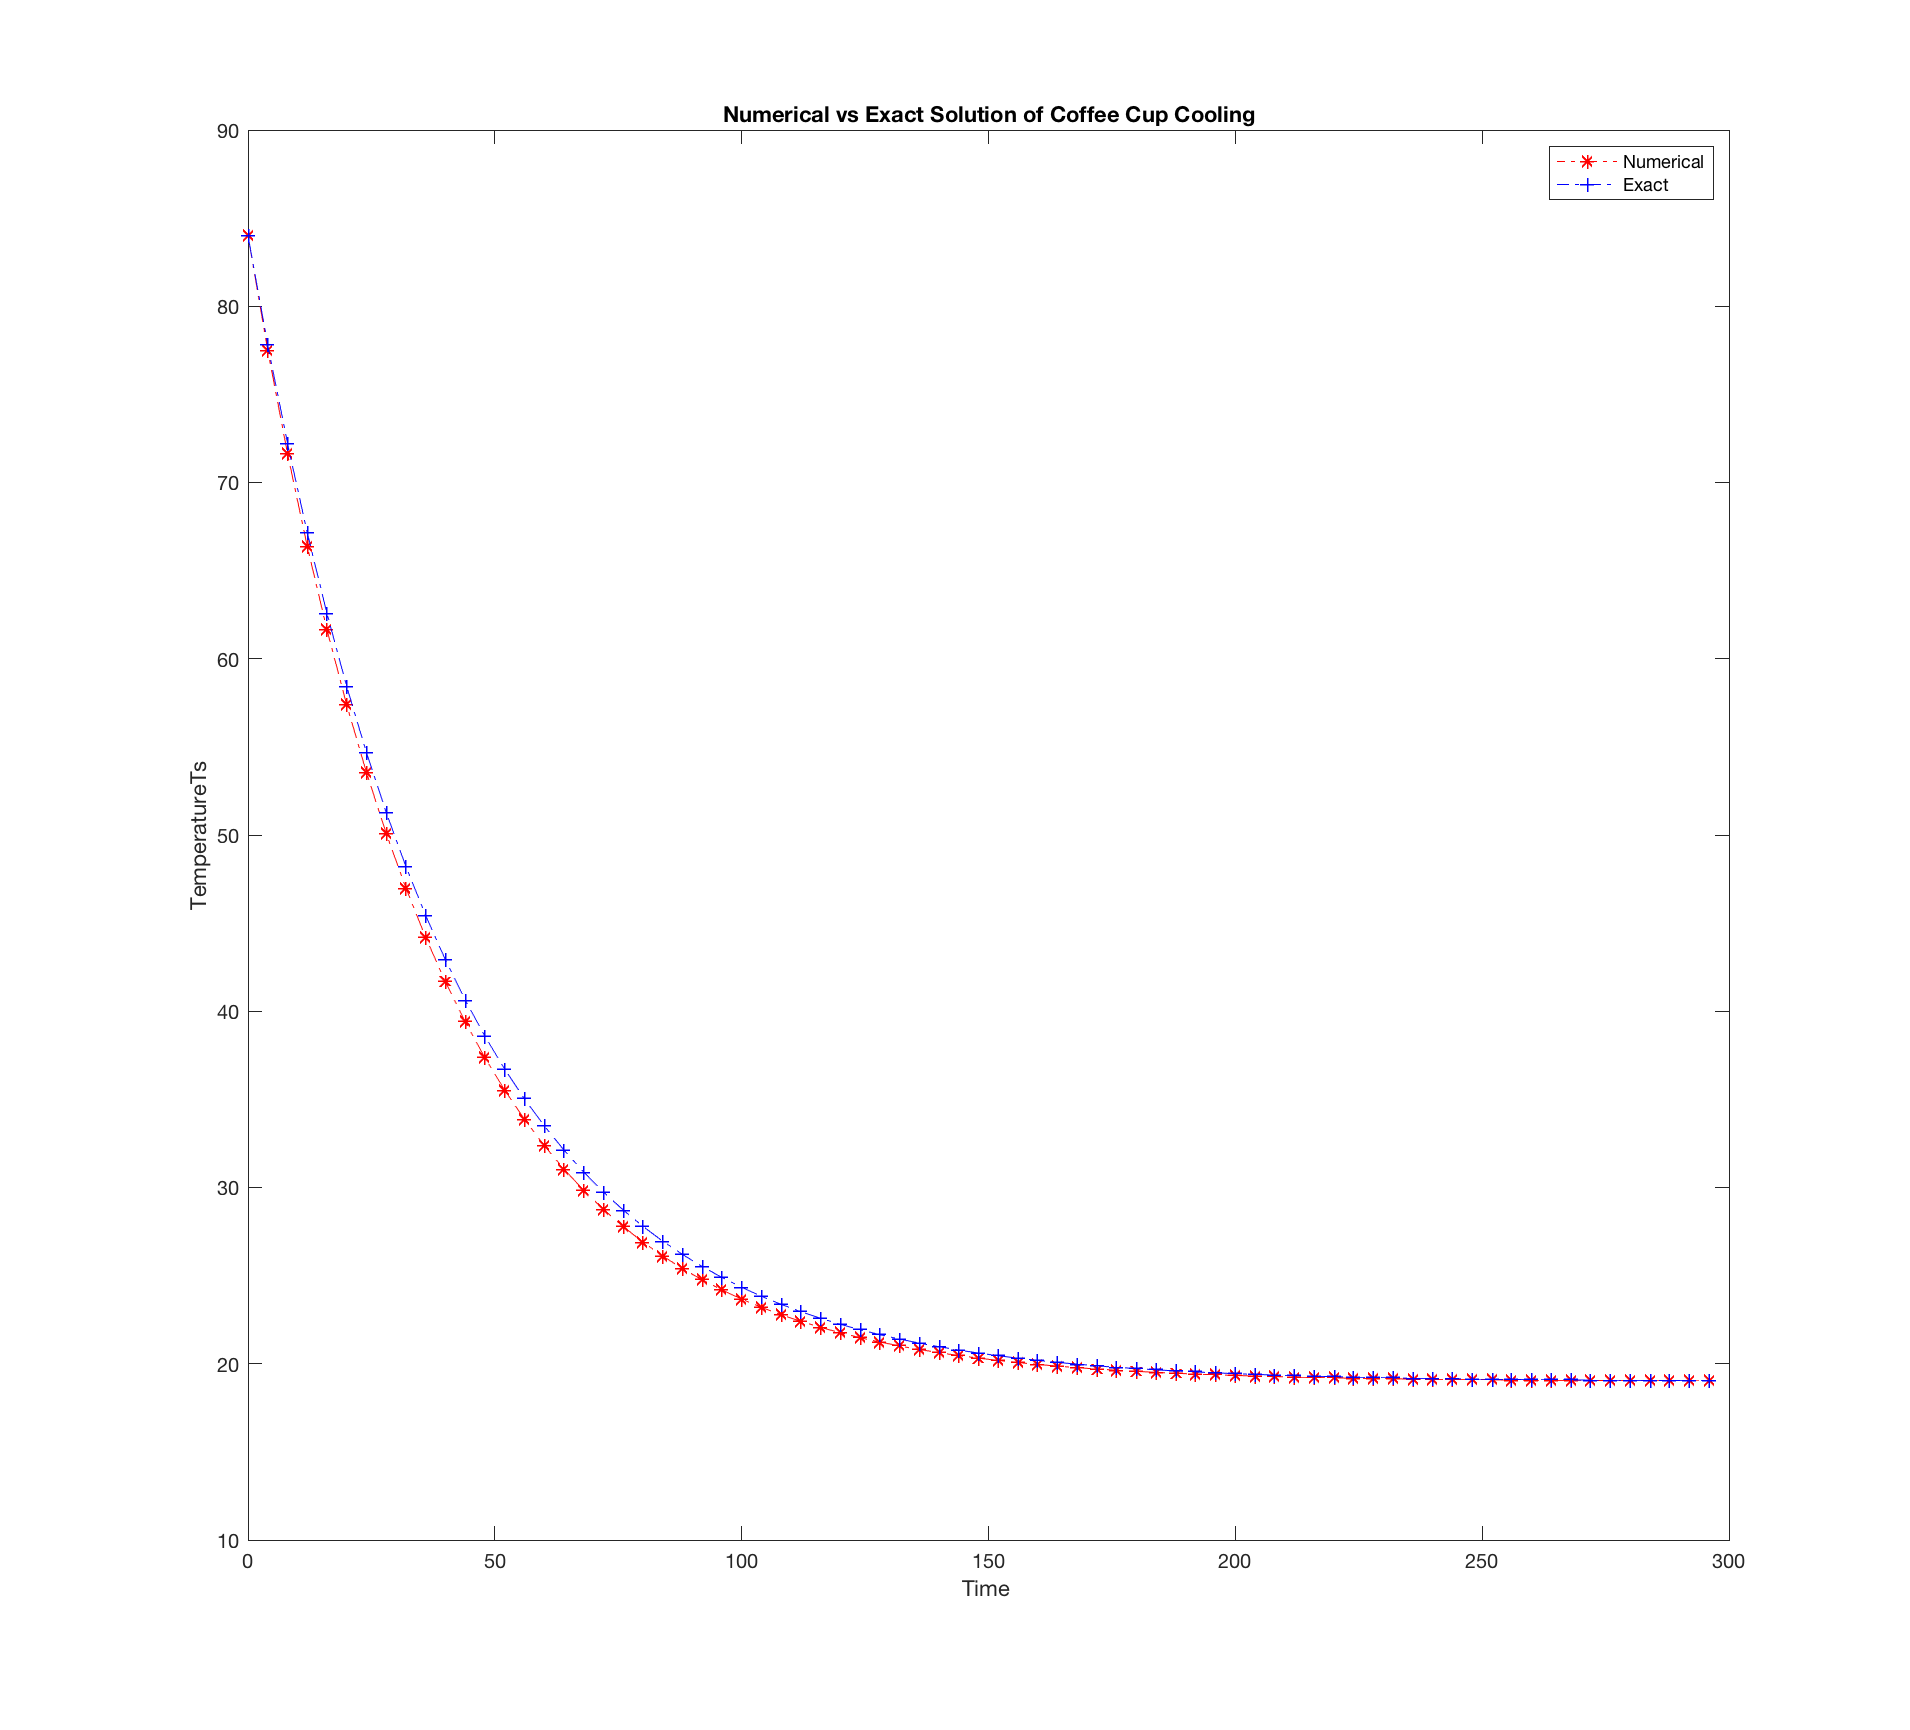
\includegraphics[scale=0.2]{num_vs_exact_cup_cool.png} \\

\clearpage

\section{}

The below plot contains two figures. \\

\noindent
The first plot showcases a comparison between the results of running the Forward Euler method to the analytic solution calculated using the \emph{Tsexact} function. As one might expect, as dt increases, the plot decreases in smoothness as the distance between samples increases. As dt decreases, so does it's corresponding line more closely resemble the exact solution. \\

\noindent
The second plot shows how the error increases as dt increases. It compares the difference in the change of the error of the first step of integration versus the final step of integration. Clearly, the first step of integration is more sensitive to an increase in dt as the rate of increase of error does seem to be quite larger than the rate of increase of error of the final step of integration.

\begin{center}
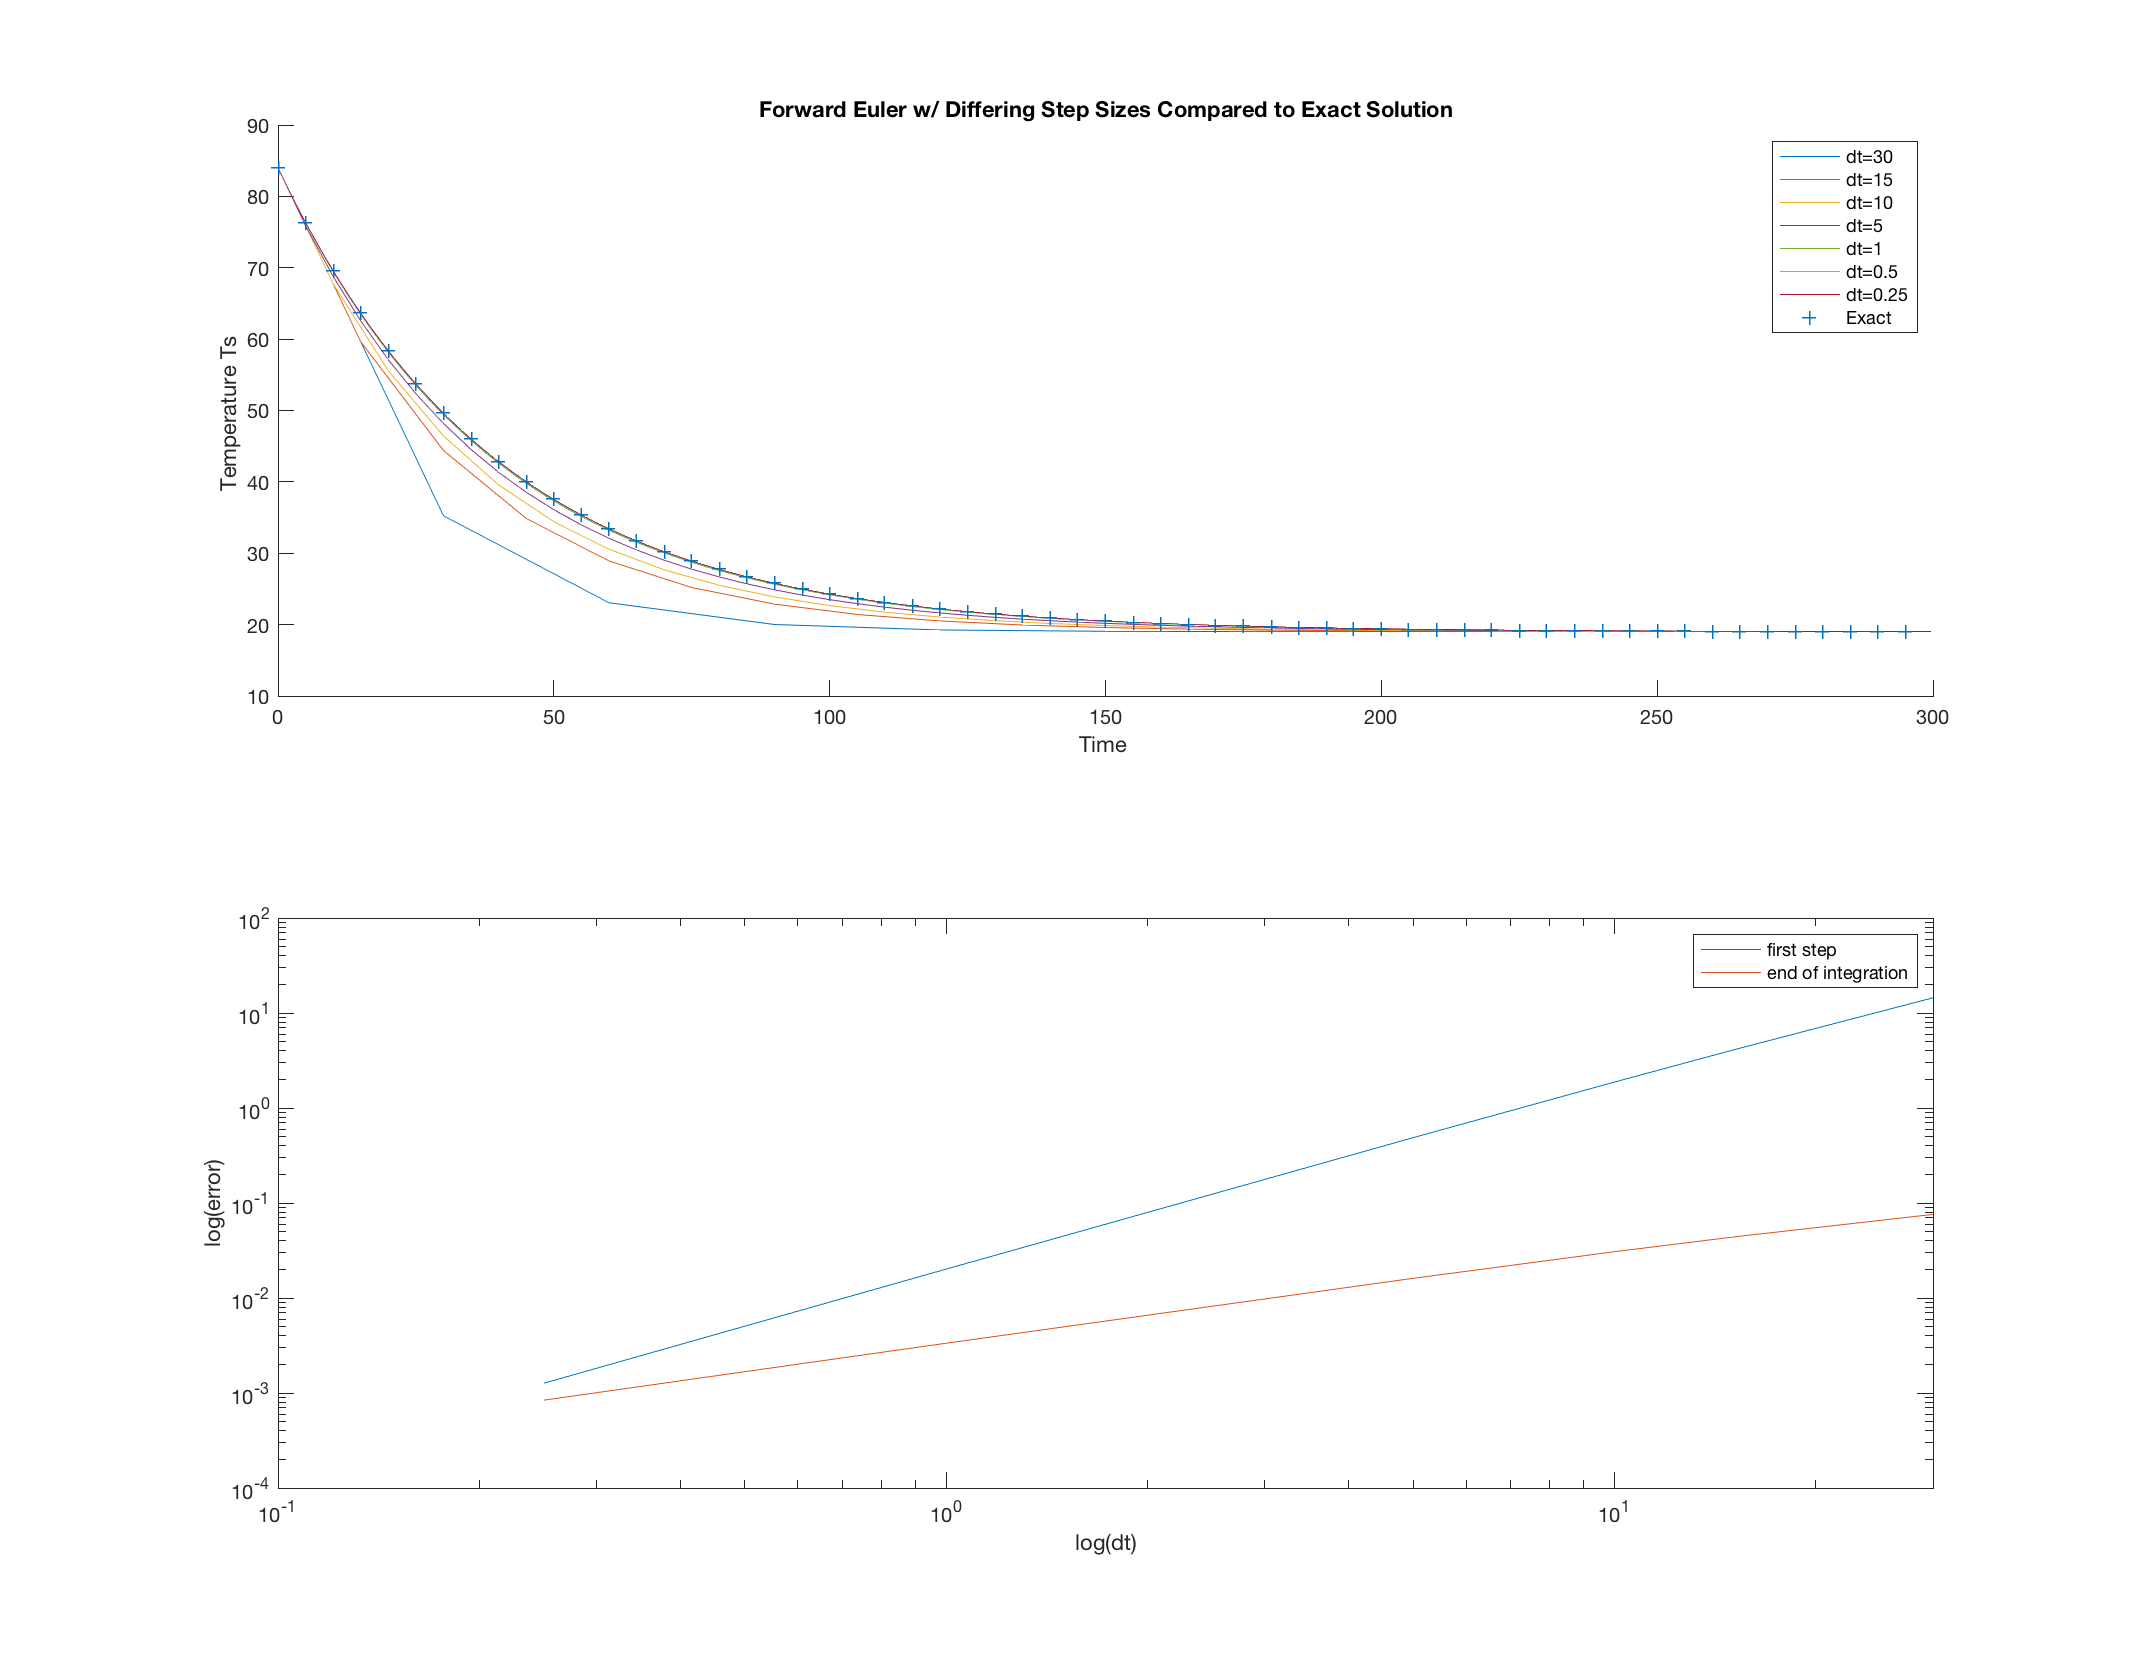
\includegraphics[scale=0.2]{for_eul_vs_exact_cup_cool.png}\\
\end{center}

\clearpage

\section{}
My implementation for the ODE23 method is in the function called \emph{ode23\_2}.

\section{}
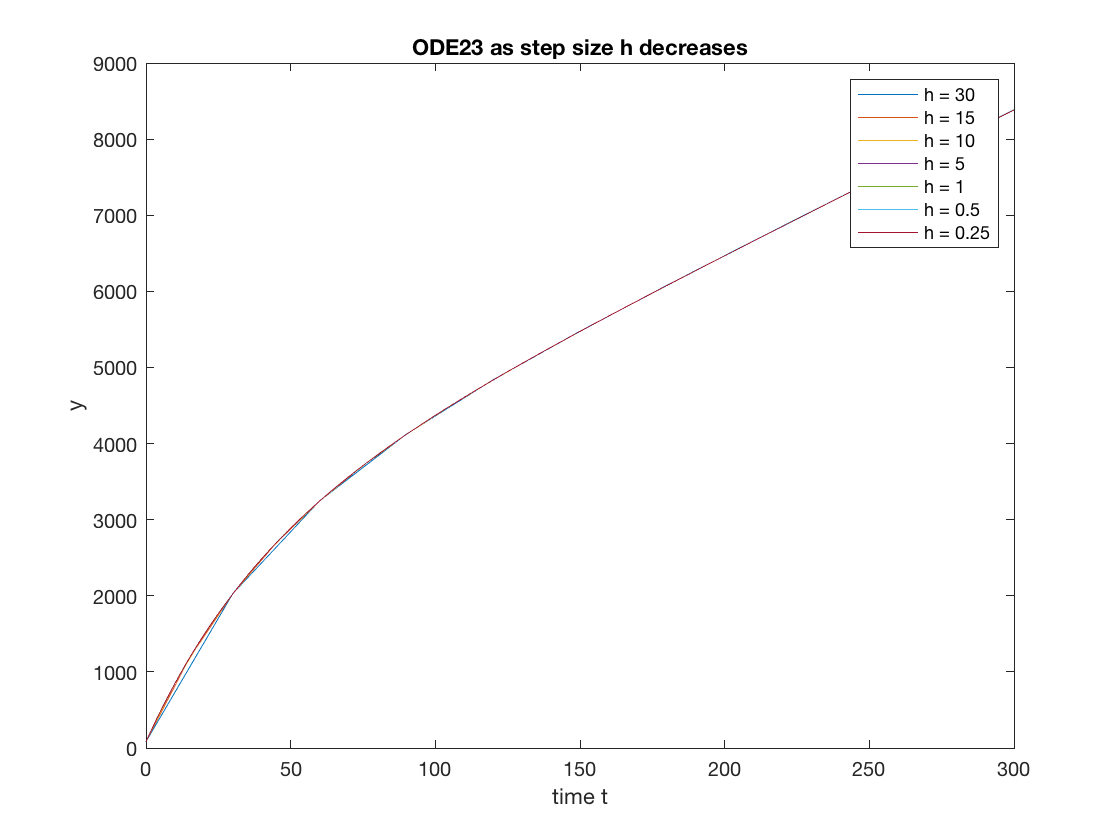
\includegraphics[scale=0.3]{fig_3.png}\\

\section{}

\section{}

Yes, in the same way as the solution becomes unstable, the error estimator also becomes unstable when r = 0.6.

\end{document}
